\chapter{k Selection in Retrieval}
\pagestyle{fancy}\lhead{\textbf \footnotesize\it{k Selection in Retrieval}}
\pagestyle{fancy}\chead{} \pagestyle{fancy}\rhead{}
\pagestyle{fancy}\lfoot{\textbf {\small\it{Univ-Mascara/Computer Science: 2025}}} 
\pagestyle{fancy}\cfoot{} \pagestyle{fancy}\rfoot{\thepage}
%%%%%%%%%%%%%%%%%%%%%%%%%%%%%%%%%%%%%%%%
\section{Introduction}
Retrieval-Augmented Generation (RAG) systems enhance language models by grounding responses in externally retrieved documents.A critical challenge in these systems is determining the optimal number of documents (k) to retrieve for a given query.Current approaches fall into three categories: static k selection, which uses a fixed number of retrieved documents; dynamic k selection, which adjusts k based on query  characteristics; and hybrid approaches, which combine both strategies.In this chapter, we first explore methods, highlighting their strengths and limitations We then introduce our novel hybrid dynamic selection algorithm provide detailed description of its methodology and present experimental results that demonstrate the effectiveness of its performance . 
%\section {The Role of k in Retrieval-Augmented Generation}
%The number of retrieved documents (k) is a critical parameter in Retrieval-Augmented Generation (RAG) that has a direct impact on the retrieval and generation phases. Choosing the right k ensures that the system retrieves enough relevant information. 
\section{Defining k: The Number of Retrieved Documents}
the parameter k denotes the number of documents or passages retrieved from an external knowledge base. This retrieval process is managed by the retriever component\cite{pareto2024rag},which identifies the top k relevant documents based on similarity to the query typically using embedding-based search\cite{Rossi_2024} (e.g., dense retrieval with FAISS, BM25, or hybrid methods) Subsequently, these documents are passed to the generator, typically a language model, which synthesizes the final response by integrating the retrieved 
\begin{figure}[h]
	\centering
	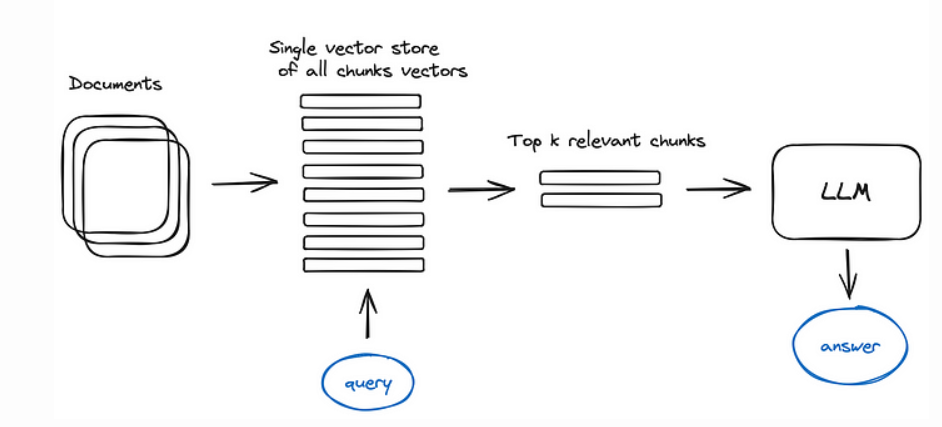
\includegraphics[width=0.9\linewidth]{Figures/topk.png}
	\caption{Basic retrieval}
	\label{rag_retrival.png}
	
\end{figure}
\newline
\section{Impact of k on Retrieval Performance}
The retriever's effectiveness in identifying relevant documents depends on k. Key impacts include :
\subsection{Recall vs. Precision} 
When a user conducts a search query, the outcomes from the database can be grouped into four distinct types based on relevance and retrieval status \cite{geeksforgeeks2022precision}:
\begin{itemize}
	\item {Relevant and Retrieved:} Documents that both address the user’s query and appear in the search results.
	\item {Relevant and Not Retrieved:} Useful documents that answer the query but are not included in the results.
	
	\item {Non-Relevant and Retrieved:} Documents that appear in the results but lack meaningful value for the query.
	 
	\item {Non-Relevant and Not Retrieved:} Irrelevant documents excluded from the results.
\end{itemize}


\textbf{Precision@k}: evaluates the proportion of relevant documents within the top k retrieved results. This metric is particularly valuable in scenarios where the focus is on delivering highly relevant information quickly, rather than ensuring complete coverage such as ,recommendation systems or search engines\cite{deconvoluteai2024metrics}.


\[
\text{Precision@k} = \frac{\text{Number of Relevant Items Retrieved in Top k}}{k}
\]

\textbf{Example}
Suppose we have a dataset of 10 documents. If we retrieve \( k = 4 \) documents and find that 3 of them are relevant to the query:

\begin{itemize}
	\item \textbf{Dataset}: [doc1, doc2, doc3, doc4, doc5, doc6, doc7, doc8, doc9, doc10]
	\item \textbf{Retrieved}: [doc3, doc1, doc7, doc4]
	\item \textbf{Relevant}: [doc1, doc3, doc5, doc8]
\end{itemize}

The Precision@4 score would be:

\[
\text{Precision@4} = \frac{3}{4} = 0.75
\]


\textbf{Recall@k :}evaluates the proportion of relevant documents that are successfully retrieved within the top k results. This metric is particularly important in contexts where ensuring the completeness of information is crucial, such as in medical research or academic tools, where omitting relevant documents could result in incomplete or inaccurate conclusions\cite{deconvoluteai2024metrics}.

\[
\text{Recall@k} = \frac{\text{Number of Relevant Items Retrieved in Top k}}{\text{Total Number of Relevant Items}}
\]
\newline
\textbf{Example}
Consider a dataset of 10 documents. If we retrieve \( k = 4 \) documents and find that 2 of them are relevant, while the total number of relevant documents in the dataset is 4:

\[
\text{Recall@4} = \frac{2}{4} = 0.5
\]


Increasing k typically enhances recall by retrieving more relevant documents but may decrease precision due to the inclusion of irrelevant ones. Conversely, decreasing k can improve precision but at the cost of lower recall. 
\subsection{Retrieval Speed and Computational Cost}
Retrieval speed and computational cost are two important areas where k has a big influence Below is a detailed explanation of how higher k values affect these aspects.

\textbf{Increased Computational Resources:} \\
As the value of k expands, the retrieval system must handle a larger set of documents, leading to higher computational demands. Specifically, the system needs to perform additional operations like ranking, filtering, and similarity scoring to identify the most relevant documents. These tasks become increasingly resource-intensive, particularly in large-scale retrieval settings where the document corpus consists of millions or even billions of entries\cite{manning2008ir}. For instance, retrieving the top  documents (k=80) requires significantly more computational resources compared to retrieving only the top 10 documents (k=5). 

\textbf{Higher Memory Usage:}
As the number of retrieved documents (k) increases ,Storing and processing a larger set of retrieved documents requires more memory This can become a significant bottleneck, especially in environments with constrained memory resources .

For large-scale retrieval tasks, where datasets may contain millions or even billions of documents, the memory demand grows proportionally with 
k. Each retrieved document needs to be stored temporarily, along with its associated metadata, such as embedding vectors, BM25 scores, or other relevance signals. Additionally, sorting and filtering operations further contribute to memory overhead
\subsection{Document Ranking Quality}
Document ranking in information retrieval involves ordering documents by their relevance to a user's query. The objective is to prioritize the most relevant documents at the top of search results, making it easier for users to access useful information quickly. Different models,Vector Space, including Boolean, and Probabilistic models, are used to establish this ranking \cite{enwiki:1262179867}.\\

Increasing the number of retrieved documents,represented as k, may result in the addition of lower-ranked, less relevant documents, potentially diluting the overall quality of the retrieved information. This occurs because of the inherent balance between precision and recall in information retrieval systems.
\begin{figure}[h]
	\centering
	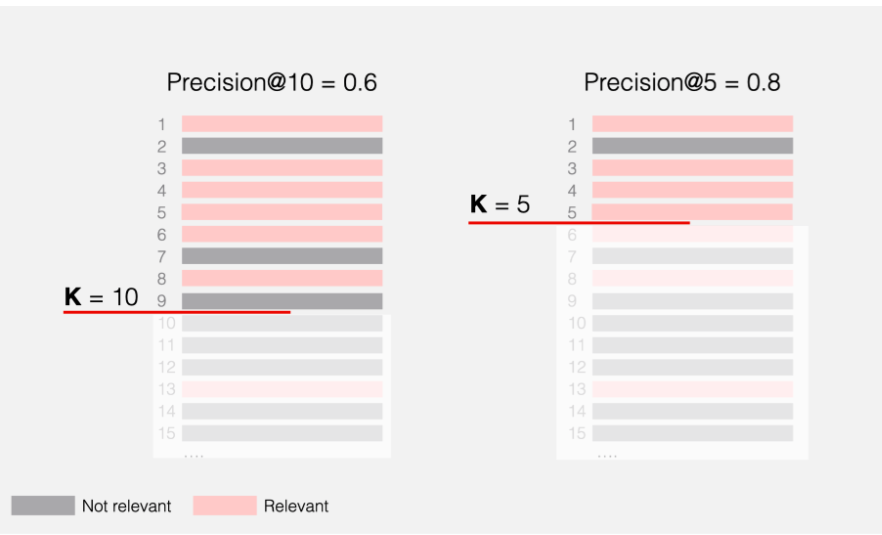
\includegraphics[width=0.7\linewidth]{Figures/precisionR.png}
	\caption{Precision in Document Ranking}
	\label{precisionR}
	
\end{figure}

\begin{figure}[h]
	\centering
	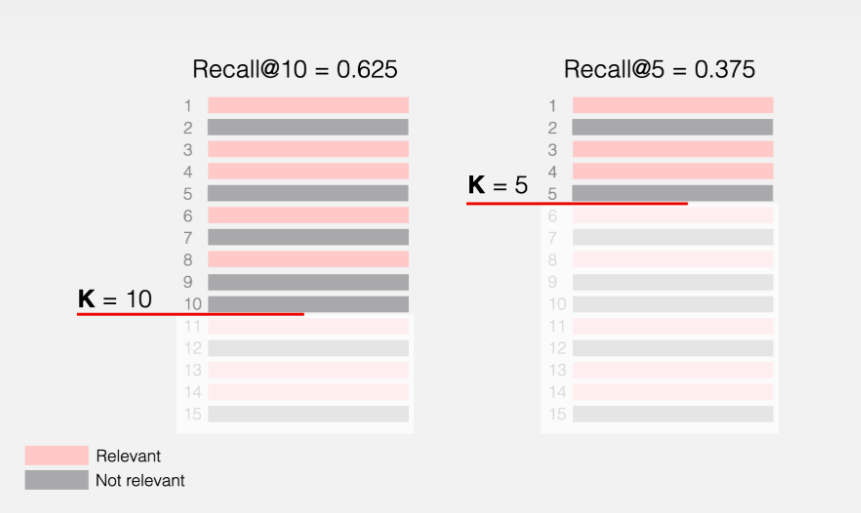
\includegraphics[width=0.7\linewidth]{Figures/recalR.png}
	\caption{Recall in Document Ranking}
	\label{recalR}
	
\end{figure}
As k grows, recall generally improves since a larger number of relevant documents are likely to be retrieved as shown in Figure \ref{recalR}. However, this often comes at the expense of precision, as the additional documents retrieved may include non-relevant ones,thereby lowering the overall precision as illustrated in Figure \ref{precisionR}. This trade-off is a core principle in evaluating information retrieval systems.

\section{Impact of k on Generation Quality}
The impact of k (the number of retrieved documents or generated candidates) on generation quality is A crucial factor in many machine learning and information retrieval tasks, including text generation, recommendation systems, and search engines . 

\subsection{Trade-off Between Diversity and Relevance} 
Higher k: Increasing k often improves diversity in generated outputs or retrieved documents, as more candidates are considered. However, this can lead to a drop in relevance or quality, as lower-ranked candidates may be less accurate or coherent. \\
Lower k: A smaller k tends to prioritize high-quality, relevant outputs but may lack diversity, leading to repetitive or overly narrow results.

Research shows that the quality of retrieved documents plays a crucial role in the performance of Retrieval-Augmented Generation (RAG) systems. For example, one study demonstrated that the precision of retrieved documents directly affects the factual correctness of the generated responses \cite{salemi2023evaluating}
Additionally, another study revealed that simply increasing the number of documents does not necessarily improve generation quality,especially if the additional documents are not highly relevant\cite{wan2025cognitivealigneddocumentselectionretrievalaugmented}
\subsection {Effect on Text Generation Models}
In text generation tasks, such as machine translation and dialogue systems, The parameter k frequently refers to the beam width in beam search algorithms\cite{freitag-al-onaizan-2017-beam}. Beam search is a heuristic search algorithm that expands the most promising nodes in a graph to maximize the quality of the text that is produced. Adjusting the beam width (k) has significantly impacts how well text generation models function.

As the beam width is increased, the model must process and retain more candidate sequences concurrently, leading to higher computational and memory demands Particularly in real-time applications where latency is crucial, this increase may have an effect on system performance and response time\cite{tensorrt_llm_beam_search}.

\section{Existing Solutions for k Selection}
Selecting an optimalnk plays a crucial role in balancing retrieval effectiveness and generation quality.Over the years, various strategies have been proposed to determine k, ranging from static selection to dynamic and hybrid approaches.
\subsection{Static k Selection}
In Retrieval-Augmented Generation (RAG) systems, "static k selection" means, refers to the process of setting a fixed number of top documents (k) to retrieve for every query, irrespective of how simple or complex the query might be. This approach simplifies the retrieval process by maintaining a consistent retrieval count across all queries

\textbf{ Sparse Retrieval with Fixed k} \\
Sparse retrieval is a method of finding relevant documents from a large collection by representing both queries and documents as vectors where most values are zero. This focus on only the most important terms leads to faster, more accurate searches, especially useful when combining information from different sources \cite{zheng2024enhancing}.

Common approaches include \textbf{BM25}\cite{10.1561/1500000019} where documents are scored for relevance by considering term frequency and inverse document frequency,it selects the 'k' documents with the highest BM25 scores for each query,\textbf{TF-IDF} (Term Frequency-Inverse Document Frequency)\cite{gfg2025tfidf}in this method the retrieved documents would be those with the highest weighted term importance, Other methods like \textbf{QLM }(Query Likelihood Model)\cite{10.1007/978-3-030-72240-1_49}use probabilistic models to evaluate the likelihood of a query and rank documents according to textual similarity.

\textbf{Dense Retrieval with Fixed k} \\
Dense retrieval \cite{karpukhin2020dense} is a method for retrieving information that uses deep learning models to convert documents and queries into high-dimensional vector embeddings,A fixed number of top-k documents are selected based on similarity scores between the query embedding and document embeddings in a continuous vector space, the retrieval process allows the system to capture semantic elationships beyond exact term matches.

Methods such as dual-encoder architectures (e.g., DPR - Dense Passage Retrieval)\cite{chen-etal-2024-dense} utilize separate neural networks (encoders) for queries and documents enable efficient retrieval, while Approximate Nearest Neighbor (ANN) search techniques (e.g., FAISS)\cite{enwiki:1276232158} optimize search efficiency in large-scale datasets .
\subsection{Dynamic k Selection}
In retrieval, dynamic k selection is the process of varying the quantity of documents (k) that are retrieved according to the properties of the query, such as its ambiguity, complexity, or relevance score distribution. This approach is crucial for enhancing the effectiveness and efficiency of information retrieval systems.

\textbf{Dynamic Trade-Off Prediction in Multi-Stage Retrieval Systems }\\ This approach predicts the optimal number of documents (k) to retrieve. It uses pre-retrieval features to balance the trade-off between retrieval efficiency and effectiveness, ensuring that the system retrieves an appropriate number of documents for each query\cite{culpepper2016dynamictradeoffpredictionmultistage}.

\textbf{Dynamic Pruning Methods:}\\
This approach addresses the challenge of balancing effectiveness and efficiency in large-scale Information Retrieval (IR) systems, particularly under temporal constraints. The goal is to process queries within a specified time limit while minimizing the loss in retrieval effectiveness. The authors propose and evaluate three techniques for temporally constrained top-K query processing \cite{10.1007/978-3-319-70145-5_1}.
\subsection{Hybrid k Selection}
hybrid methods aim to achieve optimal retrieval By merging static and dynamic k selection, These methods balance computational efficiency (from static k) with adaptive flexibility (from dynamic k) ensuring high-quality retrieval Below are some key hybrid strategies.

\textbf{Blended RAG} \\
An innovative method to improve Retrieval-Augmented Generation (RAG) systems, which integrate private document collections with Large Language Models (LLMs) for Generative Question-Answering (QA) it employs a hybrid retrieval approach, combining Dense Vector indexes and Sparse Encoder indexes with sophisticated query strategies, Blended RAG provides a scalable and efficient solution for enhancing RAG systems, showcasing the effectiveness of merging dense and sparse retrieval techniques\cite{sawarkar2024blendedragimprovingrag}.

\textbf{ STAYKATE (Static-Dynamic Hybrid Selection)} \\
A new approach for selecting in-context examples to improve the performance of large language models (LLMs) in scientific information extraction. Scientific tasks often struggle with limited training data and expensive annotation processes. STAYKATE tackles these challenges by merging static and dynamic selection strategies, combining representativeness sampling from active learning with retrieval-based methods. This hybrid approach ensures the selection of high-quality, informative examples, enhancing in-context learning for LLMs\cite{zhu2024staykatehybridincontextexample}.
\section{ Proposed Solution}
While existing k-selection approaches—static, dynamic, and hybrid—offer distinct advantages, they also present notable limitations, such as lack of adaptability in static k selection, which fails to adjust for query complexity, leading to either missing relevant documents or retrieving irrelevant ones. Dynamic k selection, while more flexible, introduces higher computational costs and requires carefully tuned heuristics, making it challenging to scale. Hybrid approaches, attempt to balance both strategies but suffer from increased system complexity.

To address these challenges, we propose an enhanced k-selection strategy that optimally balances retrieval efficiency and relevance, leveraging adaptive mechanisms to improve performance across diverse query types
\subsection{Mixture of Logits (MoL)}
\begin{figure}[h]
	\centering
	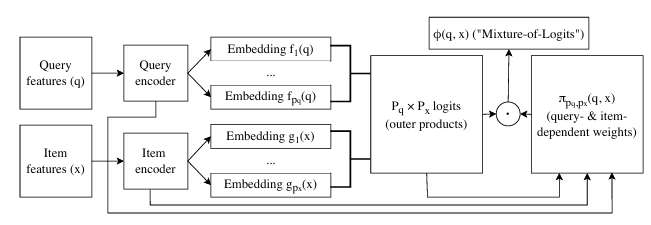
\includegraphics[width=0.7\linewidth]{Figures/mol.png}
	\caption{Mixture of Logits(MoL) learned similarity.}
	\label{Mixture_of_Logits }	
\end{figure}
The \textbf{Mixture of Logits (MoL)}\cite{zhai2023revisiting}\cite{Ding2024} approach is designed to enhance retrieval and ranking by leveraging multiple low-rank embeddings. It assumes that both the \textbf{query} (\( q \)) and \textbf{document/item} (\( x \)) are mapped into \( P \) groups of low-dimensional embeddings, denoted as \( f_p(q) \) and \( g_p(x) \), which are generated by neural networks based on their respective features.

To determine the similarity between a query and a document, MoL assigns \textbf{adaptive gating weights} \( \pi_p(q,x) \) to the inner products of these low-rank embeddings\cite{zhai2023revisiting}:

\begin{equation}
	\phi(q,x) = \sum_{p=1}^{P} \pi_p(q,x) \langle f_p(q), g_p(x) \rangle
\end{equation}

where \( \pi_p(q,x) \) represents the learned weights for each component, ensuring that their sum equals one. These weights are typically parameterized using a neural network that takes embeddings and their inner products as input features.

To efficiently scale MoL for large datasets and hardware-optimized implementations, the formulation is extended by decomposing the dot products into \textbf{batched outer products} of query-side and document-side embeddings. This decomposition improves computational efficiency, particularly on accelerators like GPUs, by normalizing the embeddings using the \( l_2 \)-norm:\cite{zhai2023revisiting}

\begin{equation}
	\phi(q,x) = \sum_{pq=1}^{P_q} \sum_{px=1}^{P_x} \pi_{pq,px}(q,x) \frac{\langle f_{pq}(q), g_{px}(x) \rangle}{|| f_{pq}(q) ||_2 || g_{px}(x) ||_2}
\end{equation}

Since embedding normalization can be precomputed, both formulations remain interchangeable in practical applications. Furthermore, it is possible to \textbf{decompose any high-rank matrix} into a mixture of logits based on low-rank matrices, demonstrating the flexibility and scalability of this approach in large-scale information retrieval tasks.
\subsection{Algorithm Design}

we introduce an adaptive threshold mechanism
(Dynamic Candidate Selection), the MoL framework is employed to refine the
candidate retrieval process. 
1. \textbf{Component-Level Embeddings}:  
Component-level embeddings are generated for all items in the dataset \(X\). These embeddings facilitate efficient similarity computations during retrieval. Formally,
\begin{equation}
	X_p \leftarrow \{g_p(x) \mid x \in X\}.
\end{equation}

\noindent
2. \textbf{Dynamic Threshold Adjustment}:  
To improve retrieval quality, \textbf{Mixture of Logits (MoL)} scores are computed for each candidate \(x \in G\). The adaptive gating weights \(\pi_p(q, x)\) allow the algorithm to dynamically adjust the retrieval threshold \(T_{\text{adaptive}}\) based on the MoL scores. The scoring function is defined as:
\begin{equation}
	\phi(q, x) = \sum_{p=1}^{P} \pi_p(q, x) \cdot \langle f_p(q), g_p(x) \rangle.
\end{equation}
The adaptive threshold \(T_{\text{adaptive}}\) is set as the minimum score among the candidates:
\begin{equation}
	T_{\text{adaptive}} = \min\{s \mid s \in G\}.
\end{equation}

\noindent
3. \textbf{Refinement and Top-K Selection}:  
Using the adaptive threshold \(T_{\text{adaptive}}\), additional relevant candidates are retrieved, expanding the candidate set \(G'\). This is achieved by including candidates whose scores exceed the threshold:
\begin{equation}
	G' \leftarrow G \cup \{x \mid s_p \geq T_{\text{adaptive}}\}.
\end{equation}
The algorithm then sorts \(G'\) based on MoL scores to select the most relevant top-k candidates.

\noindent
4. \textbf{Exact Top-K Selection}:  
Finally, the candidates in \(G'\) are sorted by their MoL scores, and the exact top-k items are extracted:
\begin{equation}
	G_{\text{final}} = \text{Top-k}(G', \phi(q, x)).
\end{equation}

\begin{figure}[ht]
	\centering
	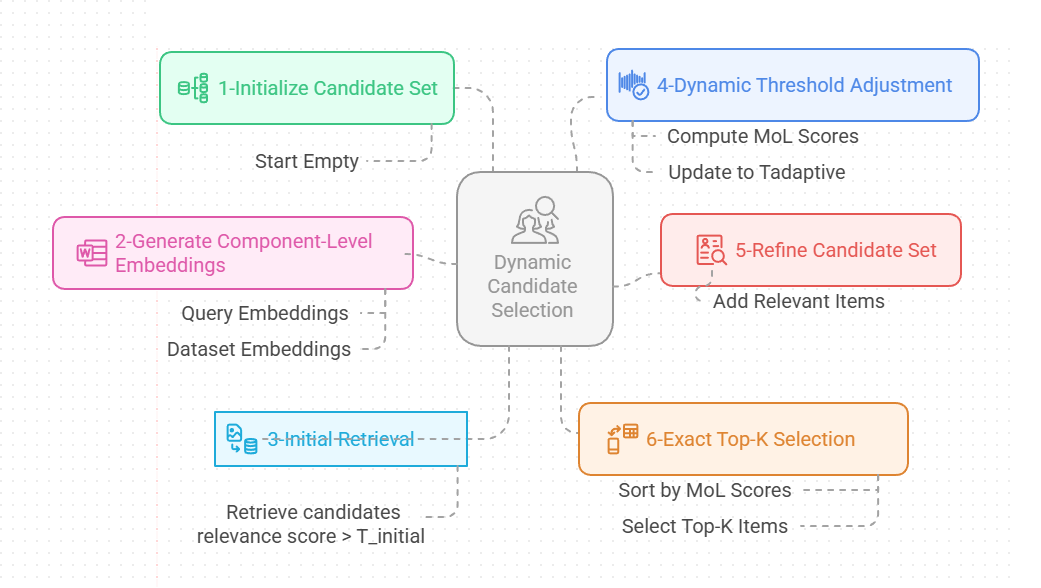
\includegraphics[width=0.7\linewidth]{Figures/propused _solution_steps.png}
	\caption{propused solution steps}
	\label{propused _solution_steps}	
\end{figure}

\subsection{Pseudocode}

\textbf{Input:} Query $q$, Set of items $X$, Component-level embeddings: $f_p(q)$, $g_p(x)$ for $p \in P$, $x \in X$, Initial threshold $T_{\text{init}}$ \\
\textbf{Output:} Exact top $k$ items based on dynamic threshold selection, $G_{\text{final}}$ \\
\SetKwInOut{Input}{Input}
\SetKwInOut{Output}{Output}

\begin{algorithm}[H]
	\small
	
	\caption{Hybrid Exact Top-k with Threshold-Based k Selection}
	\label{ALgo1}
	\SetKwProg{Init}{Initialization}{}{}
	\Init{
		$G \gets \emptyset$ \tcp{Initial candidate set}
		\ForEach{component $p \in P$}{
			$X_p \gets \{g_p(x) \mid x \in X\}$ \tcp{Precompute embeddings}
		}
	}
	

	\textbf{1. Initial Candidate Retrieval:} \\
	\ForEach{component $p \in P$}{
		Compute dot product scores: 
		\[
		S_p \gets \{ \langle f_p(q), g_p(x) \rangle : x \in X_p \}
		\]
		Retrieve items with scores $S_p \geq T_{\text{init}}$ \\
		Add these items to $G$
	}
	

	\textbf{2. Adjust k Dynamically:} \\
	\ForEach{$x \in G$}{
		Compute MoL scores $s \gets \phi(q, x)$ where:
		\[
		\phi(q, x) \gets \sum_{p=1}^{P} \pi_p(q, x) \cdot \langle f_p(q), g_p(x) \rangle
		\]
		Set $T_{\text{adaptive}} = \min \{s : s \in G\}$
	}
	
	\BlankLine
	\textbf{3. Refine Candidate Set with Adaptive k:} \\
	$G' \gets \emptyset$ \\
	\ForEach{component $p \in P$}{
		Retrieve items from $X_p$ with scores $S_p \geq T_{\text{adaptive}}$ \\
		Add these items to $G'$
	}
	

	\textbf{4. Select Exact Top-k Items:} \\
	\ForEach{component $p \in P$}{
		Compute MoL scores for all items in $G'$ \\
		Sort $G'$ by MoL scores in descending order \\
		Select the top $k$ items from $G'$ where $k$ is the number of items in $G'$ exceeding $T_{\text{adaptive}}$
	}
	

	\textbf{Return:} $G_{\text{final}}$ \tcp{Retrieve Top $k$ items from $G'$}
\end{algorithm}
\section{Recommendation System Overview}
Modern technology and online services have enabled unprecedented access to vast amounts of data. However, this abundance of information creates an overload, making it harder for users to find relevant content efficiently. Recommender systems address this by filtering information and delivering personalized suggestions, saving users time and effortz\cite{Roy2022}. These systems are now integral to platforms like e-commerce, television programs\cite{5174476}, e-learning\cite{WANG201110831}, tourism, and more, though further improvements are needed to enhance their versatility and accuracy.
\begin{figure}[ht]
	\centering
	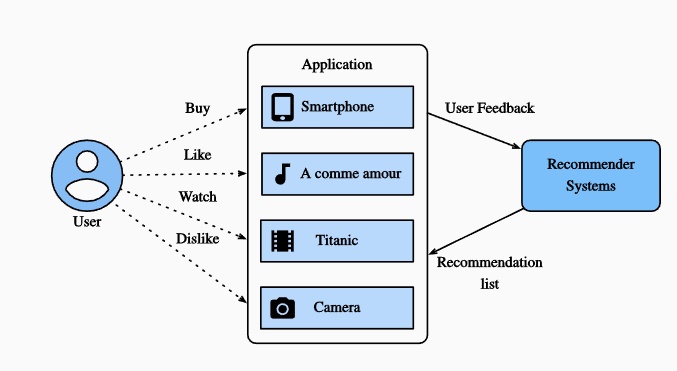
\includegraphics[width=0.5\linewidth]{Figures/RS.png}
	\caption{Recommendation System Process}
	\label{Recommendation_System _Process}	
\end{figure}
\subsection{SASRec: Self-Attentive Sequential Recommendation}
Sequential recommendation systems aim to predict a user’s next interaction based on their historical behavior while incorporating contextual information from recent actions. However, effectively capturing patterns in sequential data is challenging due to the exponential growth of the input space as more past interactions are considered.\cite{kang2018selfat}
\subsection{SASRec Model Architecture}
SASRec leverages self-attention to assign adaptive weights to past items at each time step. The key components include:\\
\textbf{ Embedding Layer:} Converts user interactions into dense vector representations. \\
\textbf{ Self-Attention Layer: }Captures dependencies between different interactions in the sequence, allowing for long-range modeling.\\
\textbf{ Point-Wise Feed Forward Network (FFN)}: Enhances feature extraction for better predictions.\\
\textbf{Prediction Layer:} Computes the likelihood of the next interaction based on learned patterns.\\
A visual representation of SASRec’s training process (Figure \ref{the_training_process_of_SASRec}) illustrates how the model uses self-attention to focus on relevant past interactions when making predictions
\begin{figure}[ht]
	\centering
	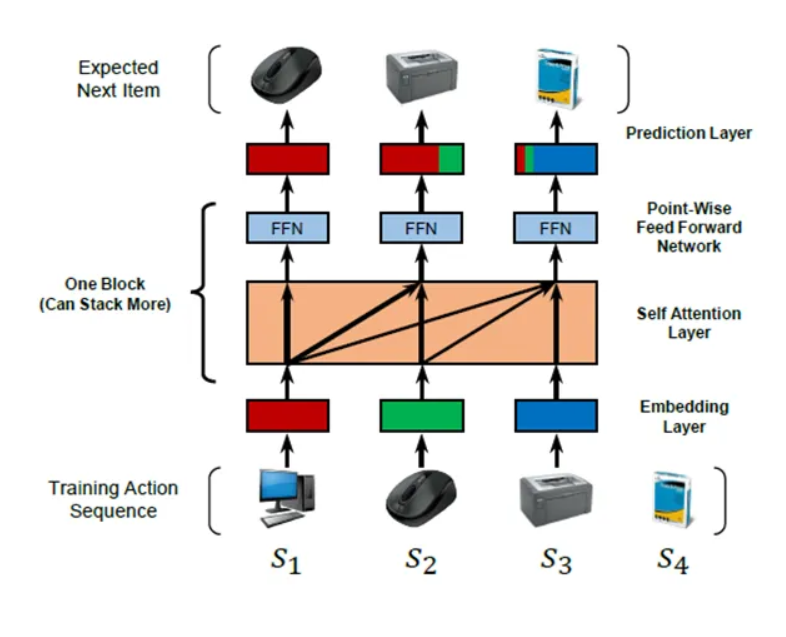
\includegraphics[width=0.6\linewidth]{Figures/sasrec.png}
	\caption{the training process of SASRec}
	\label{the_training_process_of_SASRec}	
\end{figure}
\section{Evaluation Metrics}
We employ standard ranking metrics widely used in sequential recommendation:

\begin{itemize}
	\item \textbf{Hit Rate at \( k \) (HR@\( k \))}: Measures the proportion of cases where the target item appears in the top-\( k \) recommendations. The HR@\( k \) is computed as:\cite{Tamm_2021}
	\begin{equation}
		\text{HR@}k = \frac{1}{|U|} \sum_{u=1}^{|U|} \mathbb{I}(\text{rank}_u \leq k),
	\end{equation}
	where \( |U| \) is the number of users, \( \text{rank}_u \) is the rank of the target item for user \( u \), and \( \mathbb{I}(\cdot) \) is the indicator function that returns 1 if the condition is true and 0 otherwise.
	
	\item \textbf{Mean Reciprocal Rank (MRR)}:is a ranking quality metric that measures how quickly a system retrieves the first relevant item. It is calculated as the average of reciprocal ranks across all users or queries,MRR ranges from 0 to 1, with higher values indicating better performance \cite{eviden2025mrr}.
	\begin{equation}
		\text{MRR} = \frac{1}{|U|} \sum_{u=1}^{|U|} \frac{1}{\text{rank}_u},
	\end{equation}
	where \( \text{rank}_u \) is the position of the first relevant item for user \( u \) within the top-K results. \\ 
	U represents the total number of users (for recommendation systems) or queries (for information retrieval tasks) in the dataset.
	
	\item \textbf{Normalized Discounted Cumulative Gain (NDCG)}: Assesses the ranking quality while accounting for position importance. The NDCG@\( k \) is computed as:\cite{Tamm_2021}
	\begin{equation}
		\text{NDCG@}k = \frac{1}{|U|} \sum_{u=1}^{|U|} \frac{\text{DCG@}k}{\text{IDCG@}k},
	\end{equation}
	where \( \text{DCG@}k \) is the Discounted Cumulative Gain at position \( k \):
	\begin{equation}
		\text{DCG@}k = \sum_{i=1}^{k} \frac{2^{\text{rel}_i} - 1}{\log_2(i + 1)},
	\end{equation}
	and \( \text{IDCG@}k \) is the Ideal DCG@\( k \), computed by sorting the items by their true relevance scores.
\end{itemize}  
Table \ref{tab:results_tab} summarizes the performance of our hybrid algorithm compared to the MoL-based approach on the MovieLens 100K and 1M datasets, both tested using a Max Sequence Length of 50, an Embedding Dimension of 128, 2 Attention Heads, a Feedforward Dimension of 128, a Batch Size of 128, and trained for 10 epochs 
\section{ Conclusion }
The selection of k in retrieval plays a pivotal role in balancing relevance, efficiency, and computational cost. Throughout this chapter, we explored how different approaches—static, dynamic, and hybrid—impact retrieval performance and generation quality. While static selection provides consistency, it lacks adaptability to varying query complexities. Dynamic methods introduce flexibility but come with computational overhead, whereas hybrid strategies aim to balance both. The Hybrid Exact Top-k with Threshold-Based k Selection method offers an advanced solution by leveraging adaptive weighting to enhance ranking effectiveness. Ultimately, an effective k-selection strategy is essential for optimizing retrieval systems, ensuring both efficiency and high-quality results in knowledge-augmented applications.
